    \chapter{Methodology}
       \section{SOFTWARE DEVELOPMENT APPROACH}
        Prototyping model is a type of software develpoment model. It is an iterative approach where a basic prototype is constructed to gain a better understanding of the project. This prototype is typically incomplete or lacking many components. The model is then refined based on feedback and system is reconstructed iteratively until desired conditions are met.
         \begin{figure}[hbt!]
            \center{
                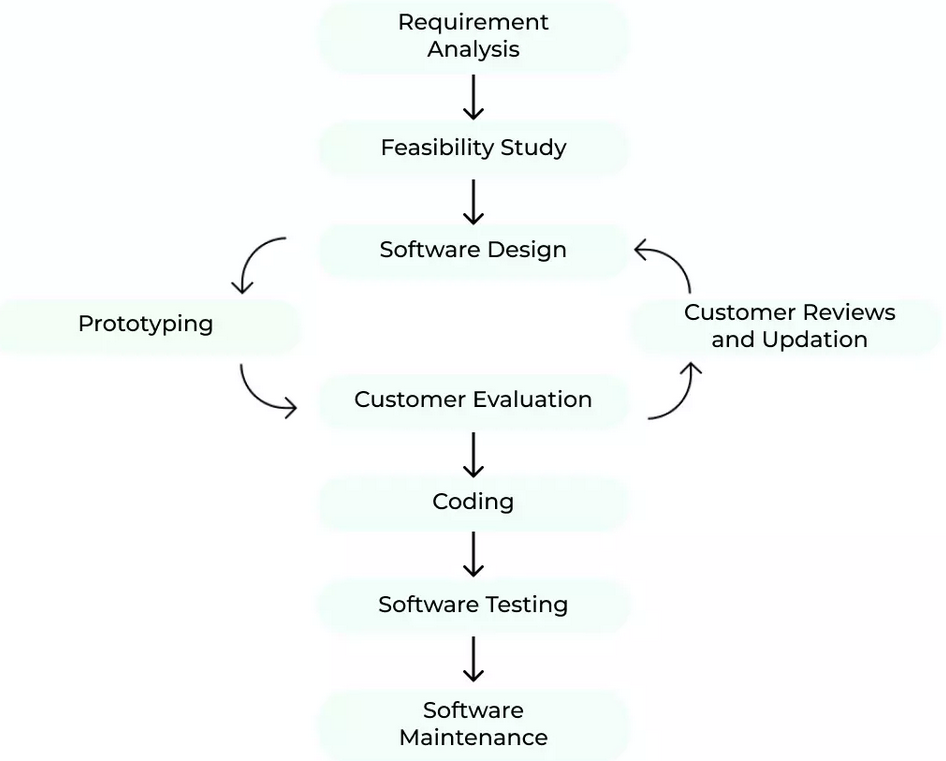
\includegraphics[width=0.75\textwidth]{./img/prototype model.png}
                \caption{Prototype Model for Software Development}
            }
        \end{figure}
        \section{DATA COLLECTION}
        To gather the dataset, authentic facial images of real individuals will be utilized and marked as "Real." Subsequently, each image will undergo a deepfake transformation using a Python script called FaceSwap, and the resulting images will be labeled as "Fake".
    
        \section{Implementation}
        Deepfake images are structured and classified into fake and real face. The data set generated is splited into training set and test set. The training set is then fed into a Deep learning model (ResNet Architecture). This model is tested whether it can identify/detect the fake face using the test data.

        \vspace{0.5in}
        \begin{figure}[hbt!]
            \center{
                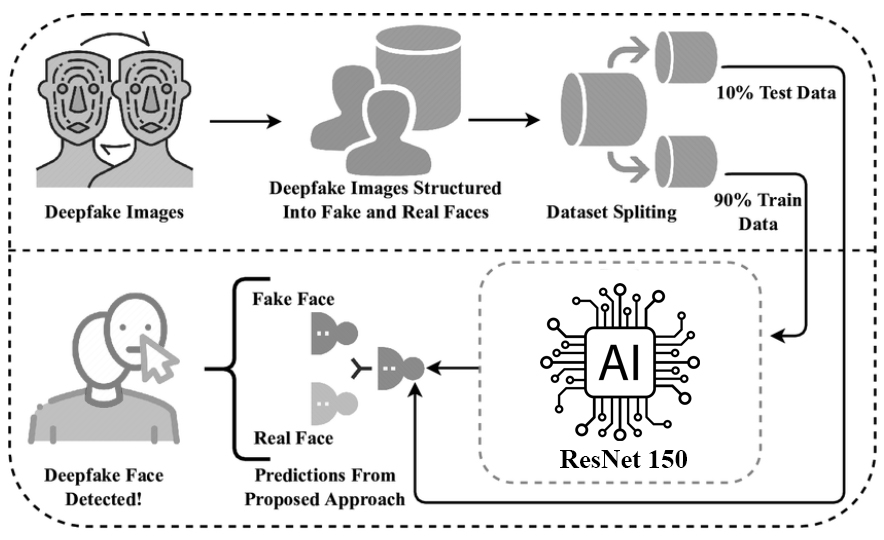
\includegraphics[width=1\textwidth]{./img/implementation.jpg}
                \caption{Methodological Architecture of Our Proposed System}
            }
        \end{figure}

        \subsection*{ResNet}
        ResNet architecture introduced the concept called Residual Blocks. In this network, we use a technique called skip connections. The skip connection connects activations of a  layer to further layers by skipping some layers in between. This forms a residual block. Resnets are made by stacking these residual blocks together. 
        The approach behind this network is instead of layers learning the underlying mapping, we allow the network to fit the residual mapping. So, instead of say H(x), initial mapping, let the network fit,
        \center{F(x) := H(x) - x 
            which gives H(x) := F(x) + x}

        \begin{figure}[hbt!]
            \center{
                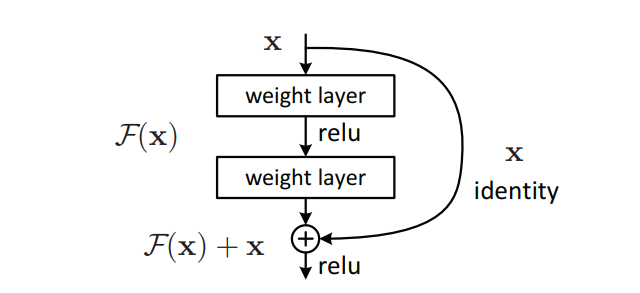
\includegraphics[width=1\textwidth]{./img/ResNet.PNG}
                \caption{Working of ResNet}
            }
        \end{figure}

        \begin{figure}
            \center{
                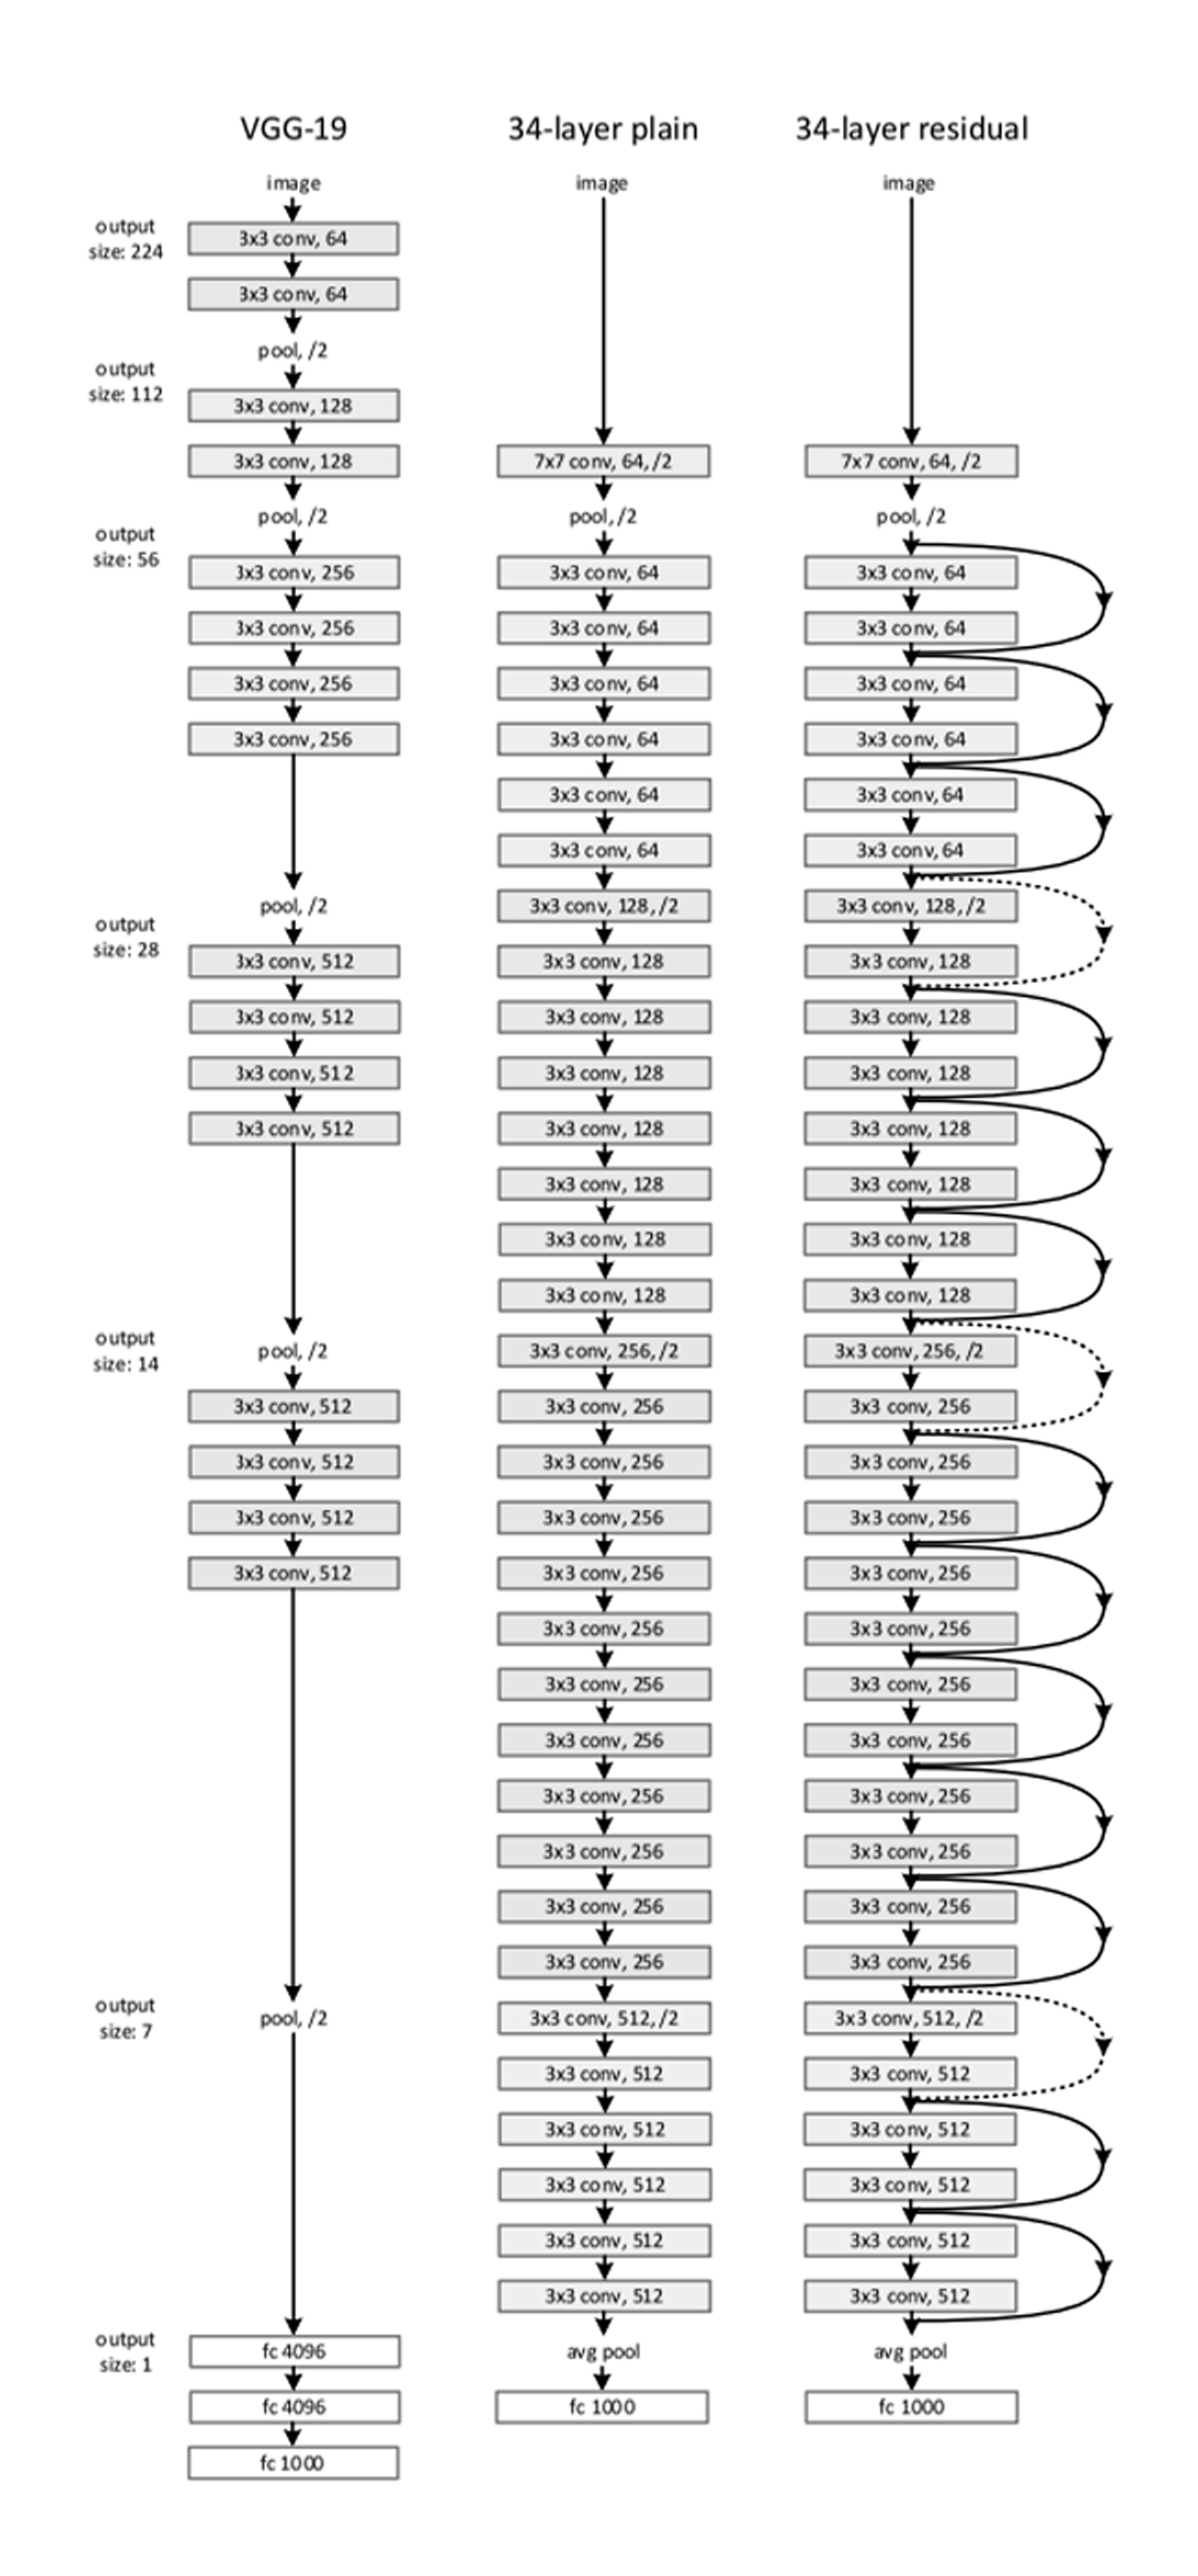
\includegraphics[height=1.4\textwidth]{./img/ResNetArc.jpg}
                \caption{ResNet Architecture}
            }
        \end{figure}

        \newpage
        \justifying
        \subsection{Gantt Chart}
            \begin{figure}[hbt!]
                \center{
                    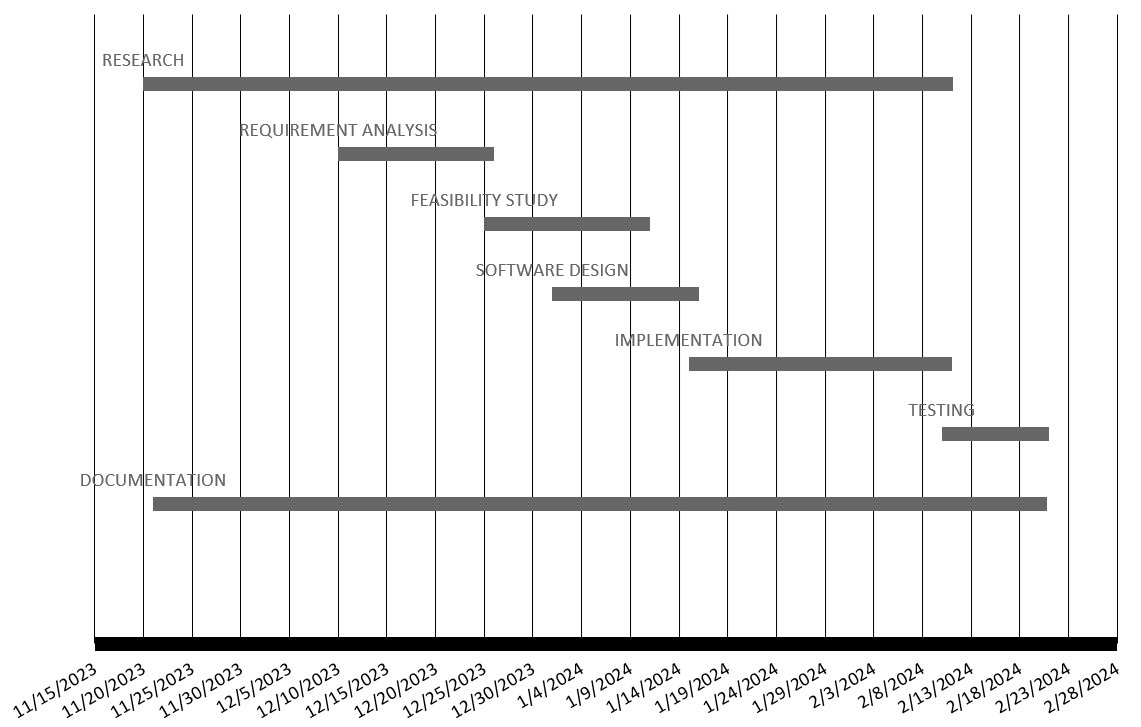
\includegraphics[width=1\textwidth]{./img/GANT_CHART.jpg}
                }
                \caption{Gantt chart}
            \end{figure}

